\documentclass[11pt, a4paper]{article}

\usepackage[margin=1in]{geometry}
\usepackage{graphicx}
\usepackage{amsmath, amssymb}
\usepackage{listings}
\usepackage{xcolor}
\usepackage{hyperref}
\usepackage{booktabs}
\usepackage{subcaption}
\usepackage{float}
\usepackage{fancyhdr}
\usepackage{enumitem}

\pagestyle{fancy}
\fancyhf{}
\fancyfoot[C]{\thepage}

\begin{document}

\fancypagestyle{no_hdr_border_rule}{
  \renewcommand{\headrulewidth}{0pt}
}
\thispagestyle{no_hdr_border_rule}

\begin{center}
    {\Large \textbf{Experiment 7 -- Report}} \\[0.2cm]
    {\large \textbf{Digital Systems and Microcontrollers (DSM)}} \\[0.1cm]
    {\normalsize International Institute of Information Technology, Hyderabad} \\[0.3cm]
\end{center}

\vspace{0.2cm}
\hrule
\vspace{0.4cm}

\noindent \textbf{Student Name 1:} Manbir Singh Judge \hfill \textbf{Roll Number:} 2026113005 \\
\noindent \textbf{Student Name 2:} Charishma Kandregula \hfill \textbf{Roll Number:} 2026112022 \\
\noindent \textbf{Table Number:} 16 \hfill \textbf{Lab Room Number:} N114 \\
\noindent \textbf{Date of Experiment:} 16/10/2026

\vspace{0.4cm}
\hrule
\vspace{0.5cm}

\vspace{1em}

\tableofcontents
\vspace{0.5cm}
\hrule
\vspace{0.8cm}

\newpage
\fancyhead[L]{Experiment 7 -- Report}
\fancyhead[R]{Part 1}

\section{Part 1 -- Decade Counter}

\subsection{Aim}
To build a circuit for decade counter.

\subsection{Components \& Equipment Required}
\begin{itemize}
    \item Digital Test Kit (DTK) -- including power supply, switches, indicator LED pairs and breadboard
    \item IC 74HC93 -- 4-bit counter
    \item IC CD4511 -- BCD to 7-segment decoder
    \item 7-segment Display
    \item Connecting Wires
\end{itemize}

\subsection{Schematic}
Following is the block diagram for decade counter using given ICs:
\begin{figure}[H]
    \centering
    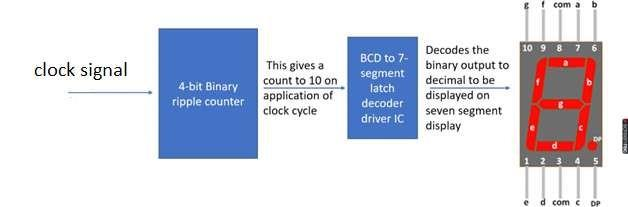
\includegraphics[width=0.8\textwidth]{block-dgm-1.png}
    \caption{Block Diagram for Decade Counter}
\end{figure}

Following are pin arrangements for used ICs:

\begin{minipage}[t]{0.48\textwidth}
\begin{figure}[H]
    \centering
    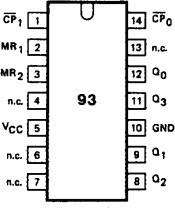
\includegraphics[width=0.6\textwidth]{ic_74hc93.png}
    \caption{Pin Arrangement for IC 74HC93}
\end{figure}
\end{minipage}
\hfill
\begin{minipage}[t]{0.48\textwidth}
\begin{figure}[H]
    \centering
    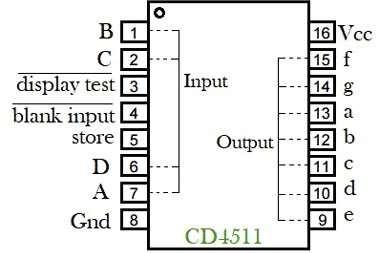
\includegraphics[width=0.8\textwidth]{ic_cd4511.png}
    \caption{Pin Arrangement for IC CD4511}
\end{figure}
\end{minipage}

\subsection{Procedure}
\begin{itemize}
    \item Place the IC 74HC93 on the breadboard and verify its operations.
    \item Repeat above step for IC CD4511.
    \item Wire the circuit according to the circuit diagram (from Tinkercad).
    \item Observe the counting on the 7-segment display and verify its correctness.
\end{itemize}

\subsection{Tinkercad Simulation}
\textbf{Tinkercad Link:} \href{https://www.tinkercad.com/things/6u4fGlekt98-dsm-experiment-7-part-1?sharecode=IUyOhaeSV8cMl_70M0GNjoGAgwwxhLYiNL1oFdGaI7M}{\color{blue}Click here}
\begin{figure}[H]
\centering
    \centering
    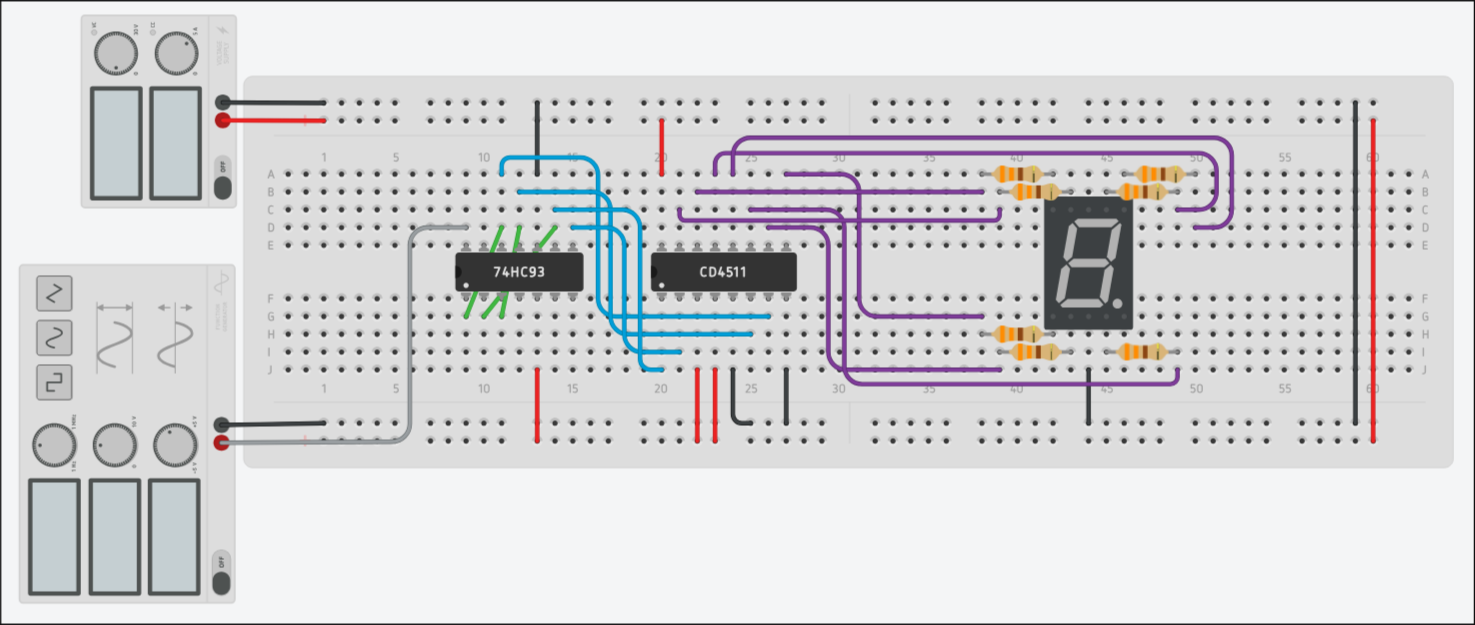
\includegraphics[width=\textwidth]{tc1.png}
    \caption{Tinkercad Simulation Screenshot}
\end{figure}

\subsection{Hardware Setup Photograph}
\begin{figure}[H]
    \centering
    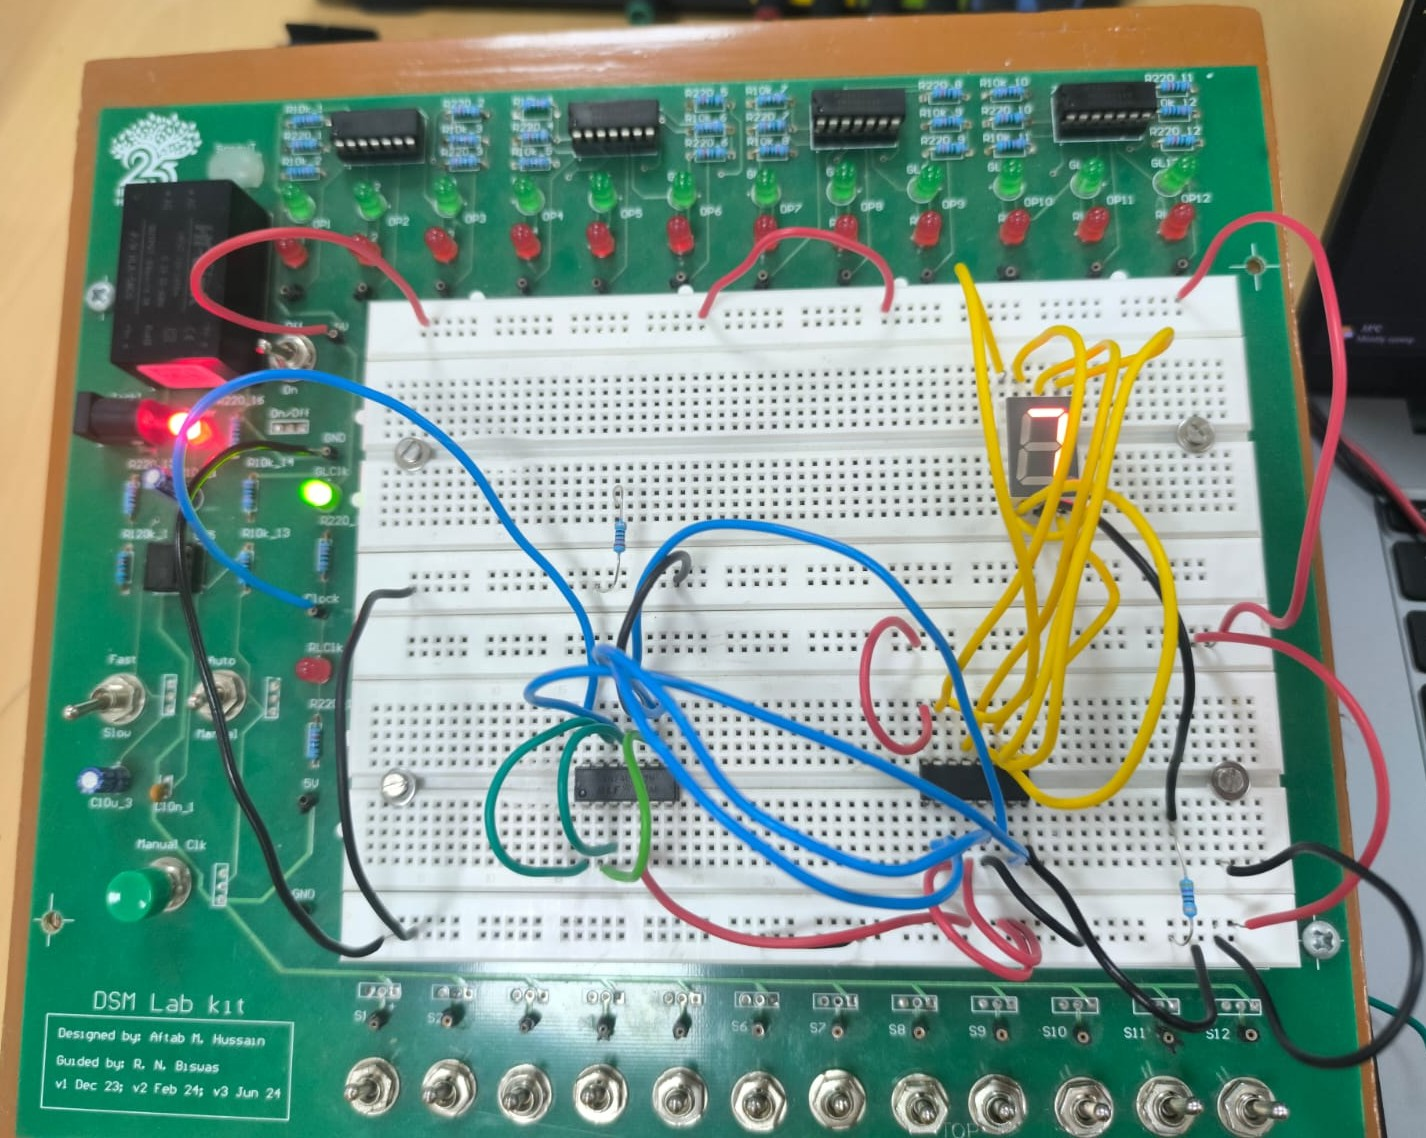
\includegraphics[width=0.6\textwidth]{lab1.jpeg}
    \caption{Physical Circuit for SR Latch}
\end{figure}

\subsection{Conclusion}
Circuit for decade counter was built.

\newpage
\fancyhead[R]{Part 2}
\section{Part 2 -- Shift Register}

\subsection{Aim}
To build a circuit for shift register and understand its usage.
\subsubsection{Part 2A}
To use the above circuit to count from 0 to 255 using Arduino.
\subsubsection{Part 2B}
To use the above circuit to take input from the user (range 0-7) and glow the corresponding LED.

\subsection{Components \& Equipment Required}
\begin{itemize}
    \item Digital Test Kit (DTK) -- including power supply, switches, indicator LED pairs, breadboard and clock
    \item IC 74HC595 -- 8-bit serial-in serial/parallel-out shift register
    \item Arduino UNO Board
    \item USB A-to-B Cable
    \item Connecting Wires
\end{itemize}

\subsection{Schematic}
Following are pin arrangements for used ICs:
\begin{figure}[H]
    \centering
    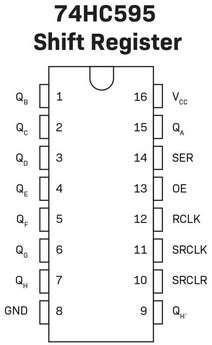
\includegraphics[width=0.2\textwidth]{ic_74hc595.png}
    \caption{Pin Arrangement for IC 74HC959}
\end{figure}

\subsection{Arduino Code}

\definecolor{vscodeBg}{rgb}{0.12, 0.12, 0.12}     
\definecolor{vscodeFg}{rgb}{0.86, 0.86, 0.86}     
\definecolor{vscodeKeyword}{rgb}{0.34, 0.61, 0.84}
\definecolor{vscodeControl}{rgb}{0.77, 0.53, 0.75}
\definecolor{vscodeString}{rgb}{0.81, 0.57, 0.47} 
\definecolor{vscodeComment}{rgb}{0.42, 0.60, 0.33}
\definecolor{vscodeNumber}{rgb}{0.71, 0.80, 0.66} 
\definecolor{vscodeLineNum}{rgb}{0.53, 0.53, 0.53}
\lstdefinestyle{customstyle}{
    backgroundcolor=\color{vscodeBg},   
    basicstyle=\ttfamily\small\color{vscodeFg},
    commentstyle=\color{vscodeComment}\itshape,
    keywordstyle=\color{vscodeKeyword}\bfseries,
    stringstyle=\color{vscodeString},
    numberstyle=\small\color{vscodeLineNum},
    breaklines=true,                 
    captionpos=b,                    
    numbers=left,                    
    numbersep=8pt,                  
    tabsize=2,
    showstringspaces=false,
    rulecolor=\color{vscodeBg}
}
\lstset{style=customstyle}

\subsubsection{Part 2A}
\begin{lstlisting}[language=C++, caption={Arduino Code for Part 2A}]
#define LATCH 8
#define DATA  9
#define CLOCK 10

void setup() {
  pinMode(LATCH, OUTPUT);
  pinMode(DATA, OUTPUT);
  pinMode(CLOCK, OUTPUT);
}

void loop() {
  for (int i = 0; i <= 255; i++) {
    digitalWrite(LATCH, LOW);
    shiftOut(DATA, CLOCK, MSBFIRST, i);
    digitalWrite(LATCH, HIGH);
    delay(500);
  }
}
\end{lstlisting}

\subsubsection{Part 2B}
\begin{lstlisting}[language=C++, caption={Arduino Code for Part 2B}]
#define LATCH 8
#define DATA  9
#define CLOCK 10

int led;

void setup() {
  Serial.begin(9600);
  pinMode(LATCH, OUTPUT);
  pinMode(DATA, OUTPUT);
  pinMode(CLOCK, OUTPUT);
}

void loop() {
  Serial.print("\nInput a number: ");
  while(Serial.available() == 0) {}
  led = Serial.read();
  led = led - '0';
  Serial.println(led);

  int cnt = (1 << led);

  digitalWrite(LATCH, LOW);
  shiftOut(DATA, CLOCK, MSBFIRST, cnt);
  digitalWrite(LATCH, HIGH);
  delay(200);
  digitalWrite(CLOCK, LOW);
}
\end{lstlisting}

\subsection{Procedure}
\begin{itemize}
    \item Place the IC 74HC595 on the breadboard and verify its operations.
    \item Connect Arduino UNO to the computer using USB A-to-B cable.
    \item Wire the circuit according to the circuit diagram (from Tinkercad).
    \item Write the above code in Arduino IDE in provided space of boiler-plate code.
    \item Compile and upload the code for Part 2A to Arduino.
    \item Observe and verify the counting.
    \item Compile and upload the code for Part 2B to Arduino.
    \item Verify that correct LED pairs light up on user input.
\end{itemize}

\subsection{Observations}
\subsubsection{Part 2A}
The connected indicator LED pairs were lighting up in sequence of counting of 8-bit binary numbers.
\subsubsection{Part 2B}
The corresponding LED pair lights up on user input.

\subsection{Tinkercad Simulation}

\subsubsection{Part 2A}
\textbf{Tinkercad Link:} \href{https://www.tinkercad.com/things/9AwTuTMx8Xo-dsm-experiment-7-part-2a?sharecode=Ri7hnk4REMBKABTiLWinTqMa_jZvVn-7bH9oRA33vfM}{\color{blue}Click here}
\begin{figure}[H]
\centering
    \centering
    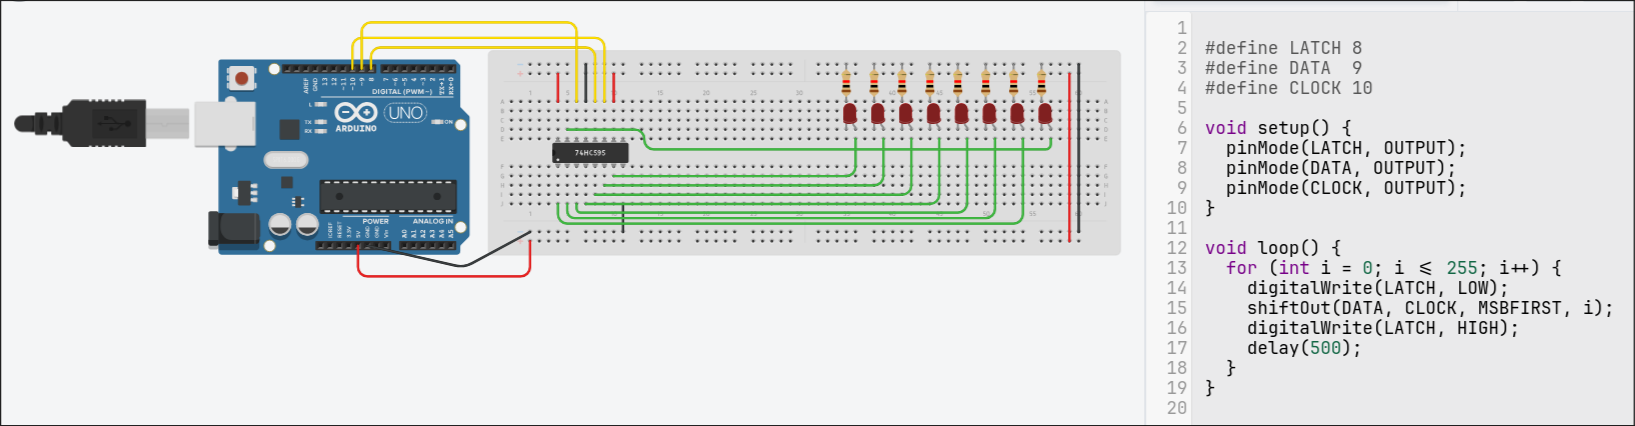
\includegraphics[width=\textwidth]{tc2.png}
    \caption{Tinkercad Simulation Screenshot}
\end{figure}

\subsubsection{Part 2B}
\textbf{Tinkercad Link:} \href{https://www.tinkercad.com/things/2c4RezSL1vs-dsm-experiment-7-part-2b?sharecode=s7PV3brBQk1aOrpG89HLcLWubMNvkNZHaAgRgKFvq3g}{\color{blue}Click here}
\begin{figure}[H]
\centering
    \centering
    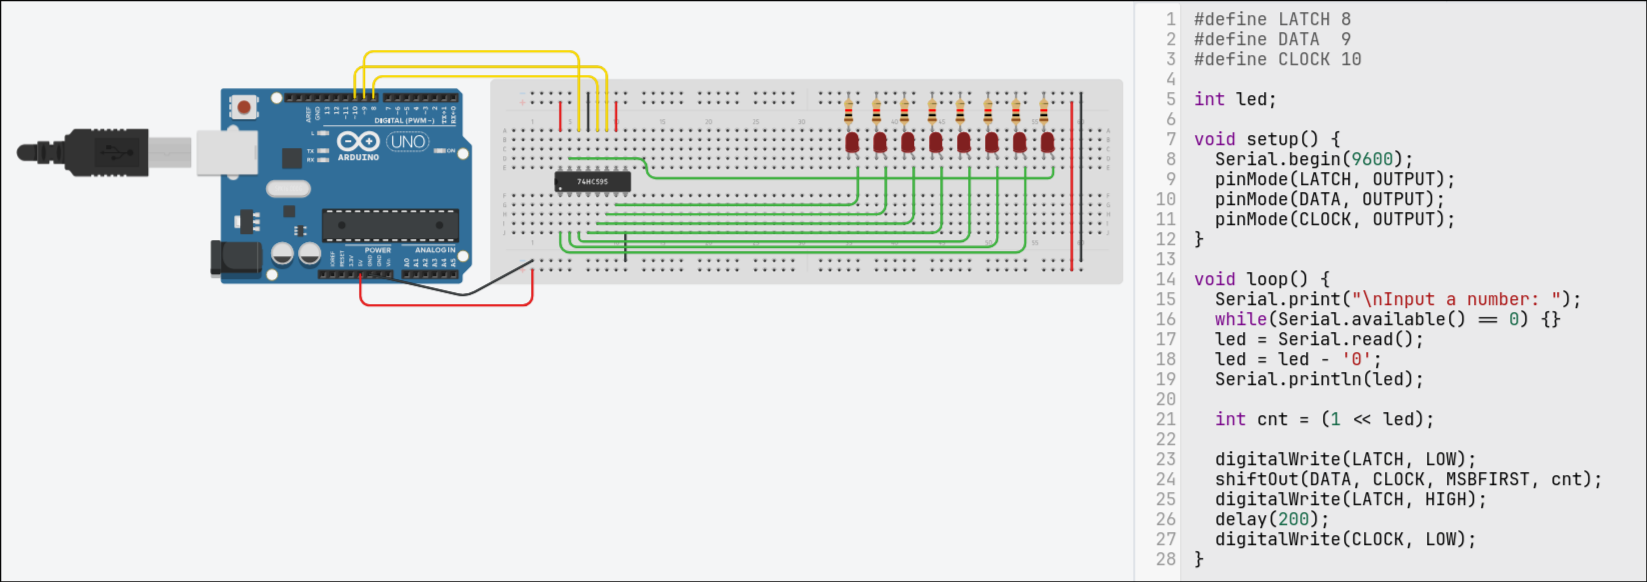
\includegraphics[width=\textwidth]{tc3.png}
    \caption{Tinkercad Simulation Screenshot}
\end{figure}

\subsection{Hardware Setup Photograph}
\begin{figure}[H]
    \centering
    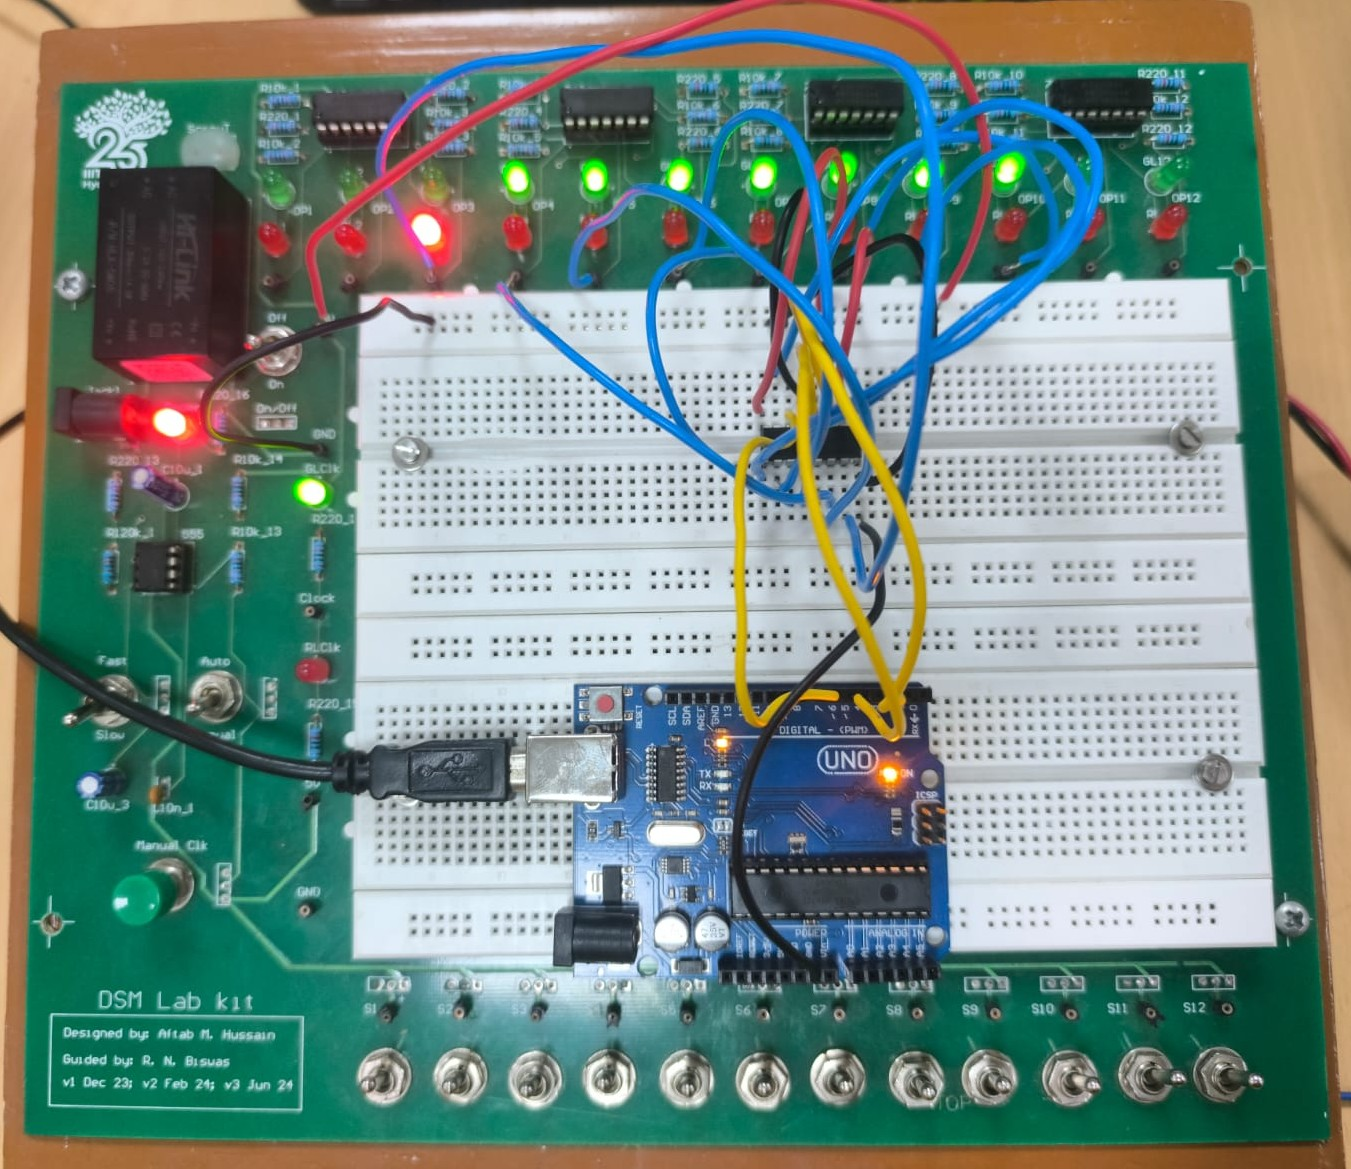
\includegraphics[width=0.6\textwidth]{lab2.jpeg}
    \caption{Hardware Setup for Shift Register}
\end{figure}

\subsection{Conclusion}
Learnt to wire and use 8-bit shift register.

\end{document}